%==============================================================================%
%                PRØVE | FORKURS 1P-2P LÆRERUTDANNING | V2018                  %
%==============================================================================%
%
% __/\\\\\\\\\\\\____________________/\\\\\\______________/\\\\\\\\\_____
%  _\/\\\////////\\\_________________\////\\\____________/\\\///////\\\___
%   _\/\\\______\//\\\___________________\/\\\___________\///______\//\\\__
%    _\/\\\_______\/\\\_____/\\\\\\\\_____\/\\\_____________________/\\\/___
%     _\/\\\_______\/\\\___/\\\/////\\\____\/\\\__________________/\\\//_____
%      _\/\\\_______\/\\\__/\\\\\\\\\\\_____\/\\\_______________/\\\//________
%       _\/\\\_______/\\\__\//\\///////______\/\\\_____________/\\\/___________
%        _\/\\\\\\\\\\\\/____\//\\\\\\\\\\__/\\\\\\\\\_________/\\\\\\\\\\\\\\\_
%         _\////////////_______\//////////__\/////////_________\///////////////_
%
%==============================================================================%
%                               MED HJELPEMIDLER                               %
%==============================================================================%
\Del*{m}


%==============================================================================%
%                                 OPPGAVE 2.1                                  %
%==============================================================================%
\Oppgave[4]

\begin{table}[H]
  \centering
  \caption{}
  \begin{tabular}{| l | *{2}{S[table-format=2.0]|}}
    \tableHeader{3}{Stortinget ved starten av perioden $2017$--$2021$}
    \Rowcolor
    Parti  \headerstrut       & {Antall kvinner} & {Antall menn} \\ \hline
    Arbeiderpartiet           &        24        &      25       \\ \hline
    Høyre                     &        20        &      25       \\ \hline
    Fremskrittspartiet        &         7        &      20       \\ \hline
    Senterpartiet             &        10        &       9       \\ \hline
    Sosialistisk Venstreparti &         4        &       7       \\ \hline
    Kristelig Folkeparti      &         2        &       6       \\ \hline
    Venstre                   &         1        &       7       \\ \hline
    Miljøpartiet De Grønne    &         1        &               \\ \hline
    Rødt                      &                  &       1       \\ \hline
  \end{tabular}
  \label{tab:Forkurs-1p-2p-laererutdanning-2018-V-oppgave-2-1}
\end{table}

\Cref{tab:Forkurs-1p-2p-laererutdanning-2018-V-oppgave-2-1} viser
stortingsrepresentantene fordelt på parti og kjønn etter stortingsvalget $2017$.

\begin{oppgaver}
  \Item{2} Legg \cref{tab:Forkurs-1p-2p-laererutdanning-2018-V-oppgave-2-1} inn
    i et regneark, og bruk regnearket til å lage et diagram som illustrerer
    opplysningene som er gitt.
\end{oppgaver}

\begin{oppgaver}
  \Item{2} Lag en ny kolonne i regnearket som viser prosentandelen kvinner i
    hvert parti.
\end{oppgaver}

\begin{figure}[H]
    \centering
    \begin{subfigure}[b]{0.31\textwidth}
      \centering
      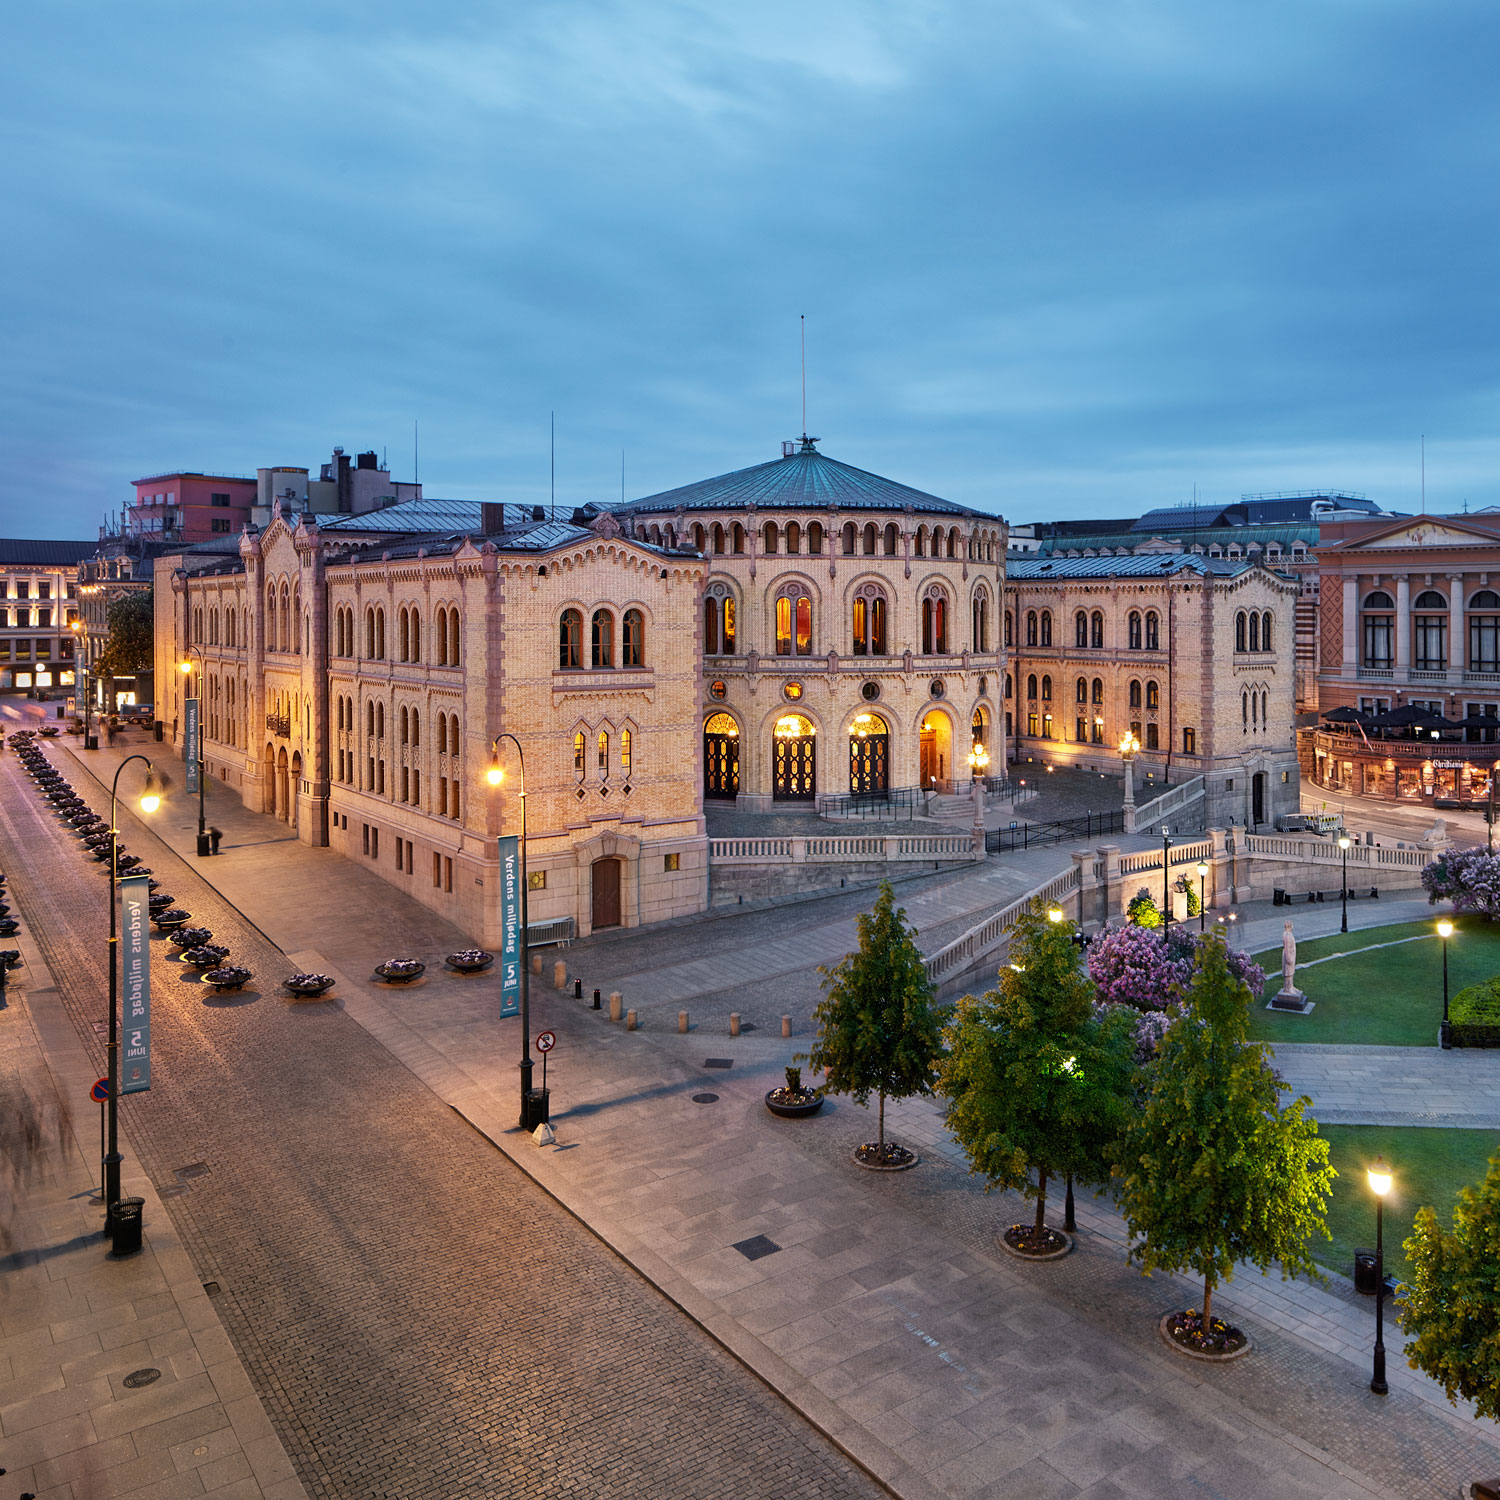
\includegraphics[trim=0 400 0 254,clip,width=\textwidth]{storting1.jpg}
    \end{subfigure}
    ~
    \begin{subfigure}[b]{0.31\textwidth}
      \centering
      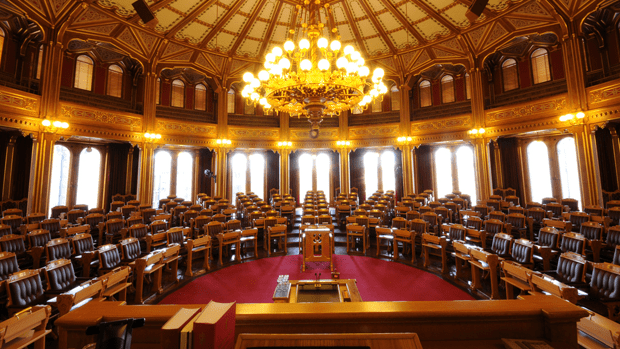
\includegraphics[width=\textwidth]{storting2.png}
    \end{subfigure}
    ~
    \begin{subfigure}[b]{0.31\textwidth}
      \centering
      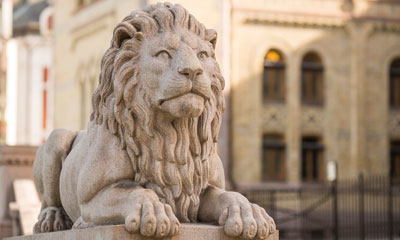
\includegraphics[trim=0 15 0 0,clip,width=\textwidth]{storting3.jpg}
    \end{subfigure}
\end{figure}


%==============================================================================%
%                                 OPPGAVE 2.2                                  %
%==============================================================================%
\Oppgave[6]

\Cref{tab:Forkurs-1p-2p-laererutdanning-2018-V-oppgave-2-2} nedenfor viser
indeksen for en vare noen år i perioden $2000$-$2017$

\begin{table}[H]
  \centering
  \caption{}
  \label{tab:Forkurs-1p-2p-laererutdanning-2018-V-oppgave-2-2}
  \begin{tabularx}{\textwidth}{|X| *{5}{Y|}}
    \hline
    \Cellcolor År     & 2000 & 2005 & 2010 & 2015 & 2017 \\
    \hline
    \Cellcolor Indeks &   74 &   99 &  105 &  100 &   97 \\
    \hline
  \end{tabularx}
\end{table}

La $x=0$ svare til år $2000$, $x=5$ til år $2005$, og så videre.

\begin{oppgaver}
  \Item{2} bruk regresjon til å vise at funksjonen $f$ er gitt ved
  %
  \begin{equation*}
    f(x) = \num{0.01} x^3 - \num{0.52}x^2 + \num{7.15}x + 75
  \end{equation*}
  %
  er en modell som passer godt med tallene i tabellen.
\end{oppgaver}

\begin{oppgaver}
  \Item{2} Bestem den gjennomsnittlige vekstfarten til funksjonen $f$ fra
    $x = 1$ til $x = 4$.  Gi en praktisk tolkning av dette svaret.
\end{oppgaver}

\begin{oppgaver}
  \Item{2} Bestem den momentane vekstfarten til funksjonen $f$ når $x = 12$.
    Gi en praktisk tolkning av dette svaret.
\end{oppgaver}


%==============================================================================%
%                                 OPPGAVE 2.3                                  %
%==============================================================================%
\Oppgave[4]

I en konfekteske er det $25$ sjokoladebiter, Jan liker $15$ av disse bitene.
Pernille tar tilfeldig to biter fra esken og gir dem til Jan.

\begin{oppgaver}
  \Item{2} Bestem sannsynligheten for at Jan liker begge bitene.
\end{oppgaver}

\begin{oppgaver}
  \Item{2} Bestem sannsynligheten for at Jan liker nøyaktig èn av bitene.
\end{oppgaver}


%==============================================================================%
%                                 OPPGAVE 2.4                                  %
%==============================================================================%
\Oppgave[4]

Anders og Lotte bruker Snapchat. Nedenfor i
\cref{fig:Forkurs-1p-2p-laererutdanning-2018-V-oppgave-2-4} ser du hvor mange
\enquote{streaks} Anders ar med ti av vennene sine.

\begin{figure}[H]
  \centering
  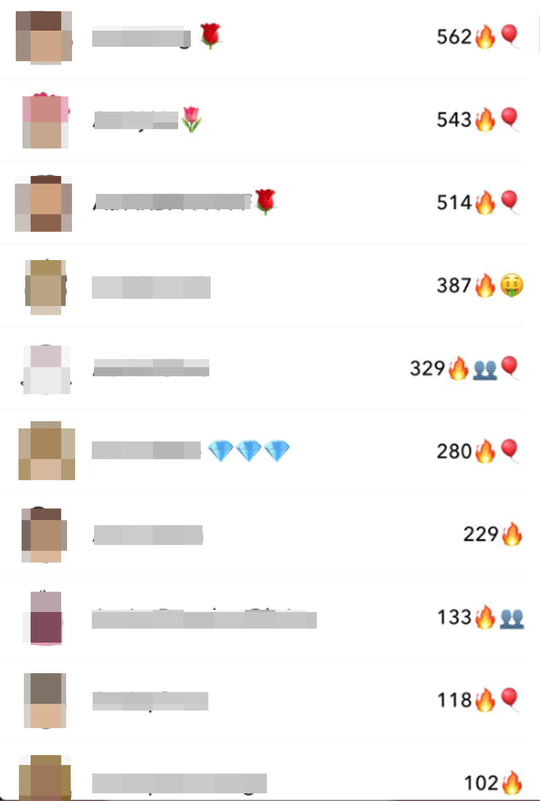
\includegraphics[width=0.6\textwidth]{Forkurs-1p-2p-laererutdanning-2018-V-oppgave-2-5-SnapChat.png}
  \caption{}
  \label{fig:Forkurs-1p-2p-laererutdanning-2018-V-oppgave-2-4}
\end{figure}

\begin{oppgaver}
  \Item{2} Bestem gjennomsnittet og standardavviket for antall
    \enquote{streaks} Anders har med disse ti vennene.
\end{oppgaver}

Lotte har beregnet gjennomsnittet og standardavviket for antall
\enquote{streaks} hun har med ti av sine venner. Hun fikk et lavere gjenomsnitt
enn Anders, men et høyere standardavvik.

\begin{oppgaver}
  \Item{2} Nedenfor er det satt opp tre påstander. Avgjør om hver enkelt
    påstand \textbf{kan} være riktig. Begrunn svarene dine.
\end{oppgaver}

\clearpage
%==============================================================================%
%                                 OPPGAVE 2.5                                  %
%==============================================================================%
\Oppgave[4]

\begin{figure}[htpb]
  \centering
  \begin{adjustbox}{width=\textwidth}
    \tikzsetnextfilename{Forkurs-1p-2p-laererutdanning-2018-V-U-oppgave-2-5}
    \begin{tikzpicture}[pics/lhead/.style={code={
          \draw[fill=maincolorMedium,even odd rule] (0,0) -- (-3,-4) -- (-3,-1) arc(270:0:3) (-3,0) rectangle (-1,2);
      }}%
      ]
      \draw[gray, dashed] (-6.5,-4.5) grid (6.5,5.5);
      \path[fill opacity=0.4] (0,0) pic{lhead} pic[xscale=-1]{lhead};
    \end{tikzpicture}
  \end{adjustbox}
  \caption{}
  \label{fig:Forkurs-1p-2p-laererutdanning-2018-V-oppgave-2-5}
\end{figure}

I \cref{fig:Forkurs-1p-2p-laererutdanning-2018-V-oppgave-2-5} ovenfor ser du en
figur tegnet på et rutenett. Anta at hver rute er kvadratisk med side
$\SI{1}{\cm}$.

\begin{oppgaver}
  \Item{2} Bestem arealet av det fargelagte området.
\end{oppgaver}

\begin{oppgaver}
  \Item{2} Bestem omkretsen av det fargelagte området.
\end{oppgaver}


%==============================================================================%
%                                 OPPGAVE 2.6                                  %
%==============================================================================%
\Oppgave[6]

For nøyaktig fem år siden satte Kari inn $\num{25000}$~kroner på en sparekontor.
Pengene har stått urørt. Kontoen har en fast årlig rente på
$\SI{2.5}{\percent}$.

\begin{oppgaver}
  \Item{2} Hvor mye har Kari på sparekonto i dag?
\end{oppgaver}

Kari vurderer å la pengene fortsatt stå urørt på kontoen.

\begin{oppgaver}
  \Item{2} Hvor mange år vil det da gå fra hun satte inn pengene, til hun har
    $\num{50000}$~kroner på konto om fire år?
\end{oppgaver}

Kari bestemmer seg for å sette inn mer penger på kontoen.

\begin{oppgaver}
  \Item{2} Hvor mye må hun sette inn på sparekontoen i dag for at det skal stå
    $\num{50000}$~kroner på kontoen om $4$~år?
\end{oppgaver}


%==============================================================================%
%                                 OPPGAVE 2.7                                  %
%==============================================================================%
\Oppgave[3]

\begin{center}\hspace*{0.5cm}
  \begin{minipage}[c]{0.3\textwidth}
    \centering\raisebox{\dimexpr \topskip-\height}{%
    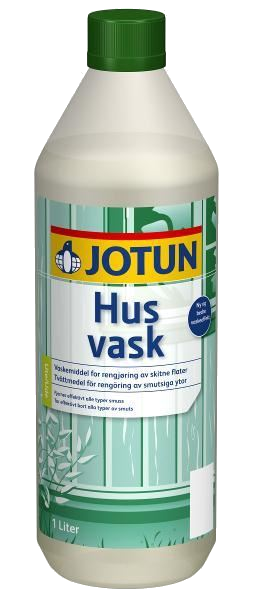
\includegraphics[scale=0.3]{Forkurs-1p-2p-laererutdanning-2018-V-oppgave-2-7-Jotun-husvask.png}}
  \end{minipage}\hfill
  \begin{minipage}[c]{0.65\textwidth}
    \section*{Blandeforhold (volum)}
    $1 : 20$ \\
    $\SI{1}{\liter}$ JOTUN Husvask til $\SI{20}{\liter}$ vann.
  \end{minipage}\bigskip
\end{center}

Jotun Husvask skal blandes med vann i forholdet $1:20$.

\begin{oppgaver}
  \Item{1} Lars har en bøtte med $\SI{5}{\L}$ vann. Hvor mange desiliter må
    han tilsette?
\end{oppgaver}

Lise har $\SI{6.3}{\L}$ ferdig blanding i forholdet $1:20$, men ønsker å
tilsette mer Husvask slit at blandingsforholdet blir $1:15$.

\begin{oppgaver}
  \Item{2} Hvor mange desiliter Husvask må hun tilsette?
\end{oppgaver}


%==============================================================================%
%                                 OPPGAVE 2.8                                  %
%==============================================================================%
\Oppgave[5] \points*{5}

\begin{table}[htbp]
  \centering
  \caption{}
  \begin{tabular}{|l| S[table-format=4.0]
                    | S[table-format=6.0]
                   l| S[table-format=6.0]
                   l|}
    \hline \Rowcolor
    Navn   &
    {Fødselsår} &
    \multicolumn{2}{c|}{\vtop{\hbox{\strut Årslønn i $2017$}\hbox{\strut
   inkludert feriepenger}}} & \multicolumn{2}{c|}{Feriepenger i $2017$} \\
   \hline
   Mari   & 1970    &  734567 & kroner  &  76661 & kroner \\ \hline
   Morten & 1998    &  430124 & kroner  &  45972 & kroner \\ \hline
   Stein  & 1982    &  649345 & kroner  &  66540 & kroner \\ \hline
   Inger  & 1957    &  385433 & kroner  &  40902 & kroner \\ \hline
          &         &         &         &        &        \\
 \end{tabular}
 \label{tab:Forkurs-1p-2p-laererutdanning-2018-V-oppgave-2-8a}
\end{table}

I \cref{tab:Forkurs-1p-2p-laererutdanning-2018-V-oppgave-2-8a} ovenfor ser du de
første linjene i en tabell fra regnskapsavdelingen i en bedrift. \bigskip

Lag et regneark som vist i
\cref{tab:Forkurs-1p-2p-laererutdanning-2018-V-oppgave-2-8b} nedenfor. Registrer
opplysningene fra tabellen i de hvite cellene i regnearket, og sett inn formler
i de fargede cellene. \bigskip

\begin{table}[H]
  \centering
  \caption{Caption}
  \label{tab:Forkurs-1p-2p-laererutdanning-2018-V-oppgave-2-8b}
  \begin{adjustbox}{center}
    \scriptsize
    \begin{tabular}{|l|M{0.04\textwidth}|
        M{0.09\textwidth}|
        M{0.133\textwidth}|
        M{0.12\textwidth}|
        M{0.12\textwidth}|
        M{0.06\textwidth}|
        M{0.12\textwidth}|
      M{0.12\textwidth}|}

      \hhline{*{9}{-}}
      \dgr{$\triangle$}
    &\mcdg{A} &\mcdg{B} &\mcdg{C} &\mcdg{D} &\mcdg{E} &\mcdg{F} &\mcdg{G} &\mcdg{H}
    \\
    \hhline{*{9}{-}}
    \midc
    &\mig{}
    &\tableTitle
    \\
    \hhline{|-|*{6}{>{\arrayrulecolor{lightGray}}-}|}
    \arrayrulecolor{black}
    \midc
    &\blviii{}
    \\
    \hhline{|-|>{\arrayrulecolor{lightGray}}->{\arrayrulecolor{black}}--|>{\arrayrulecolor{lightGray}}---|}
    \arrayrulecolor{black}
    \midc
    &\lgr
    & \cellcolor{lightGray} \textbf{År}
    &% white cell
    &\blv{}
    \\
    \hhline{|-|>{\arrayrulecolor{lightGray}}->{\arrayrulecolor{black}}--|>{\arrayrulecolor{lightGray}}---|}
    \arrayrulecolor{black}
    \midc
    &\blviii{}
    \\
    \hhline{|-|>{\arrayrulecolor{lightGray}}->{\arrayrulecolor{black}}------|>{\arrayrulecolor{lightGray}}-|}
    \arrayrulecolor{black}
    \midc
    &\lgr
    &\tableLong{Feriepengesats for arbeidstakere under $60$~år}
    &% white cell
    &\cellcolor{lightGray}
    \\
    \hhline{|-|>{\arrayrulecolor{lightGray}}->{\arrayrulecolor{black}}------|>{\arrayrulecolor{lightGray}}-|}
    \arrayrulecolor{black}
    \midc
    &\lgr
    &\tableLong{Feriepengesats for arbeidstakere over $60$~år}
    &% white cell
    &\cellcolor{lightGray}
    \\
    \hhline{|-|>{\arrayrulecolor{lightGray}}->{\arrayrulecolor{black}}------|>{\arrayrulecolor{lightGray}}-|}
    \arrayrulecolor{black}
    \midc
    &\blviii{}
    \\
    \hline
    \arrayrulecolor{black}
    \midc
    &\cellcolor{lightGray}\!\!\!\textbf{Navn}%
    &\cellcolor{lightGray}\!\!\textbf{Fødselsår}%
    &\cellcolor{lightGray}\!\!\textbf{Årslønn i $2017$ inkludert feriepenger}%
    &\cellcolor{lightGray}\!\!\textbf{Feriepenger i $2017$}%
    &\cellcolor{lightGray}\!\textbf{Feriepenge-grunnlag for $2018$}%
    &\cellcolor{lightGray}\textbf{Alder}%
    &\cellcolor{lightGray}\!\!\textbf{Feriepenge-sats}%
    &\cellcolor{lightGray}\!\!\textbf{Feriepenger i $2018$}%
    \\
    \hline
    \arrayrulecolor{black}
    \midc
    \whiteAndColorRows
    \\
    \hline
    \arrayrulecolor{black}
    \midc
    \whiteAndColorRows
    \\
    \hline
    \arrayrulecolor{black}
    \midc
    \whiteAndColorRows
    \\
    \hline
    \arrayrulecolor{black}
    \midc
    \whiteAndColorRows
      \end{tabular}
    \end{adjustbox}
\end{table}

Feriepengesatsen er $\SI{12.0}{\percent}$ for arbeidstakere under $60$ år og
$\SI{14.3}{\percent}$ for arbeidstakere over $60$ år.



